\chapter{System Design}

The System Design phase defines the overall architecture, database organisation, and workflow of the SmartSec platform. The design is based on a modular client-server architecture with six independent backend modules and a single-page React frontend.

\section{Entity Relationship (ER) Diagram}
The ER Diagram represents the logical structure of the SmartSec PostgreSQL database hosted on Supabase. It shows seven core entities and their relationships.

\begin{figure}[H]
    \centering
    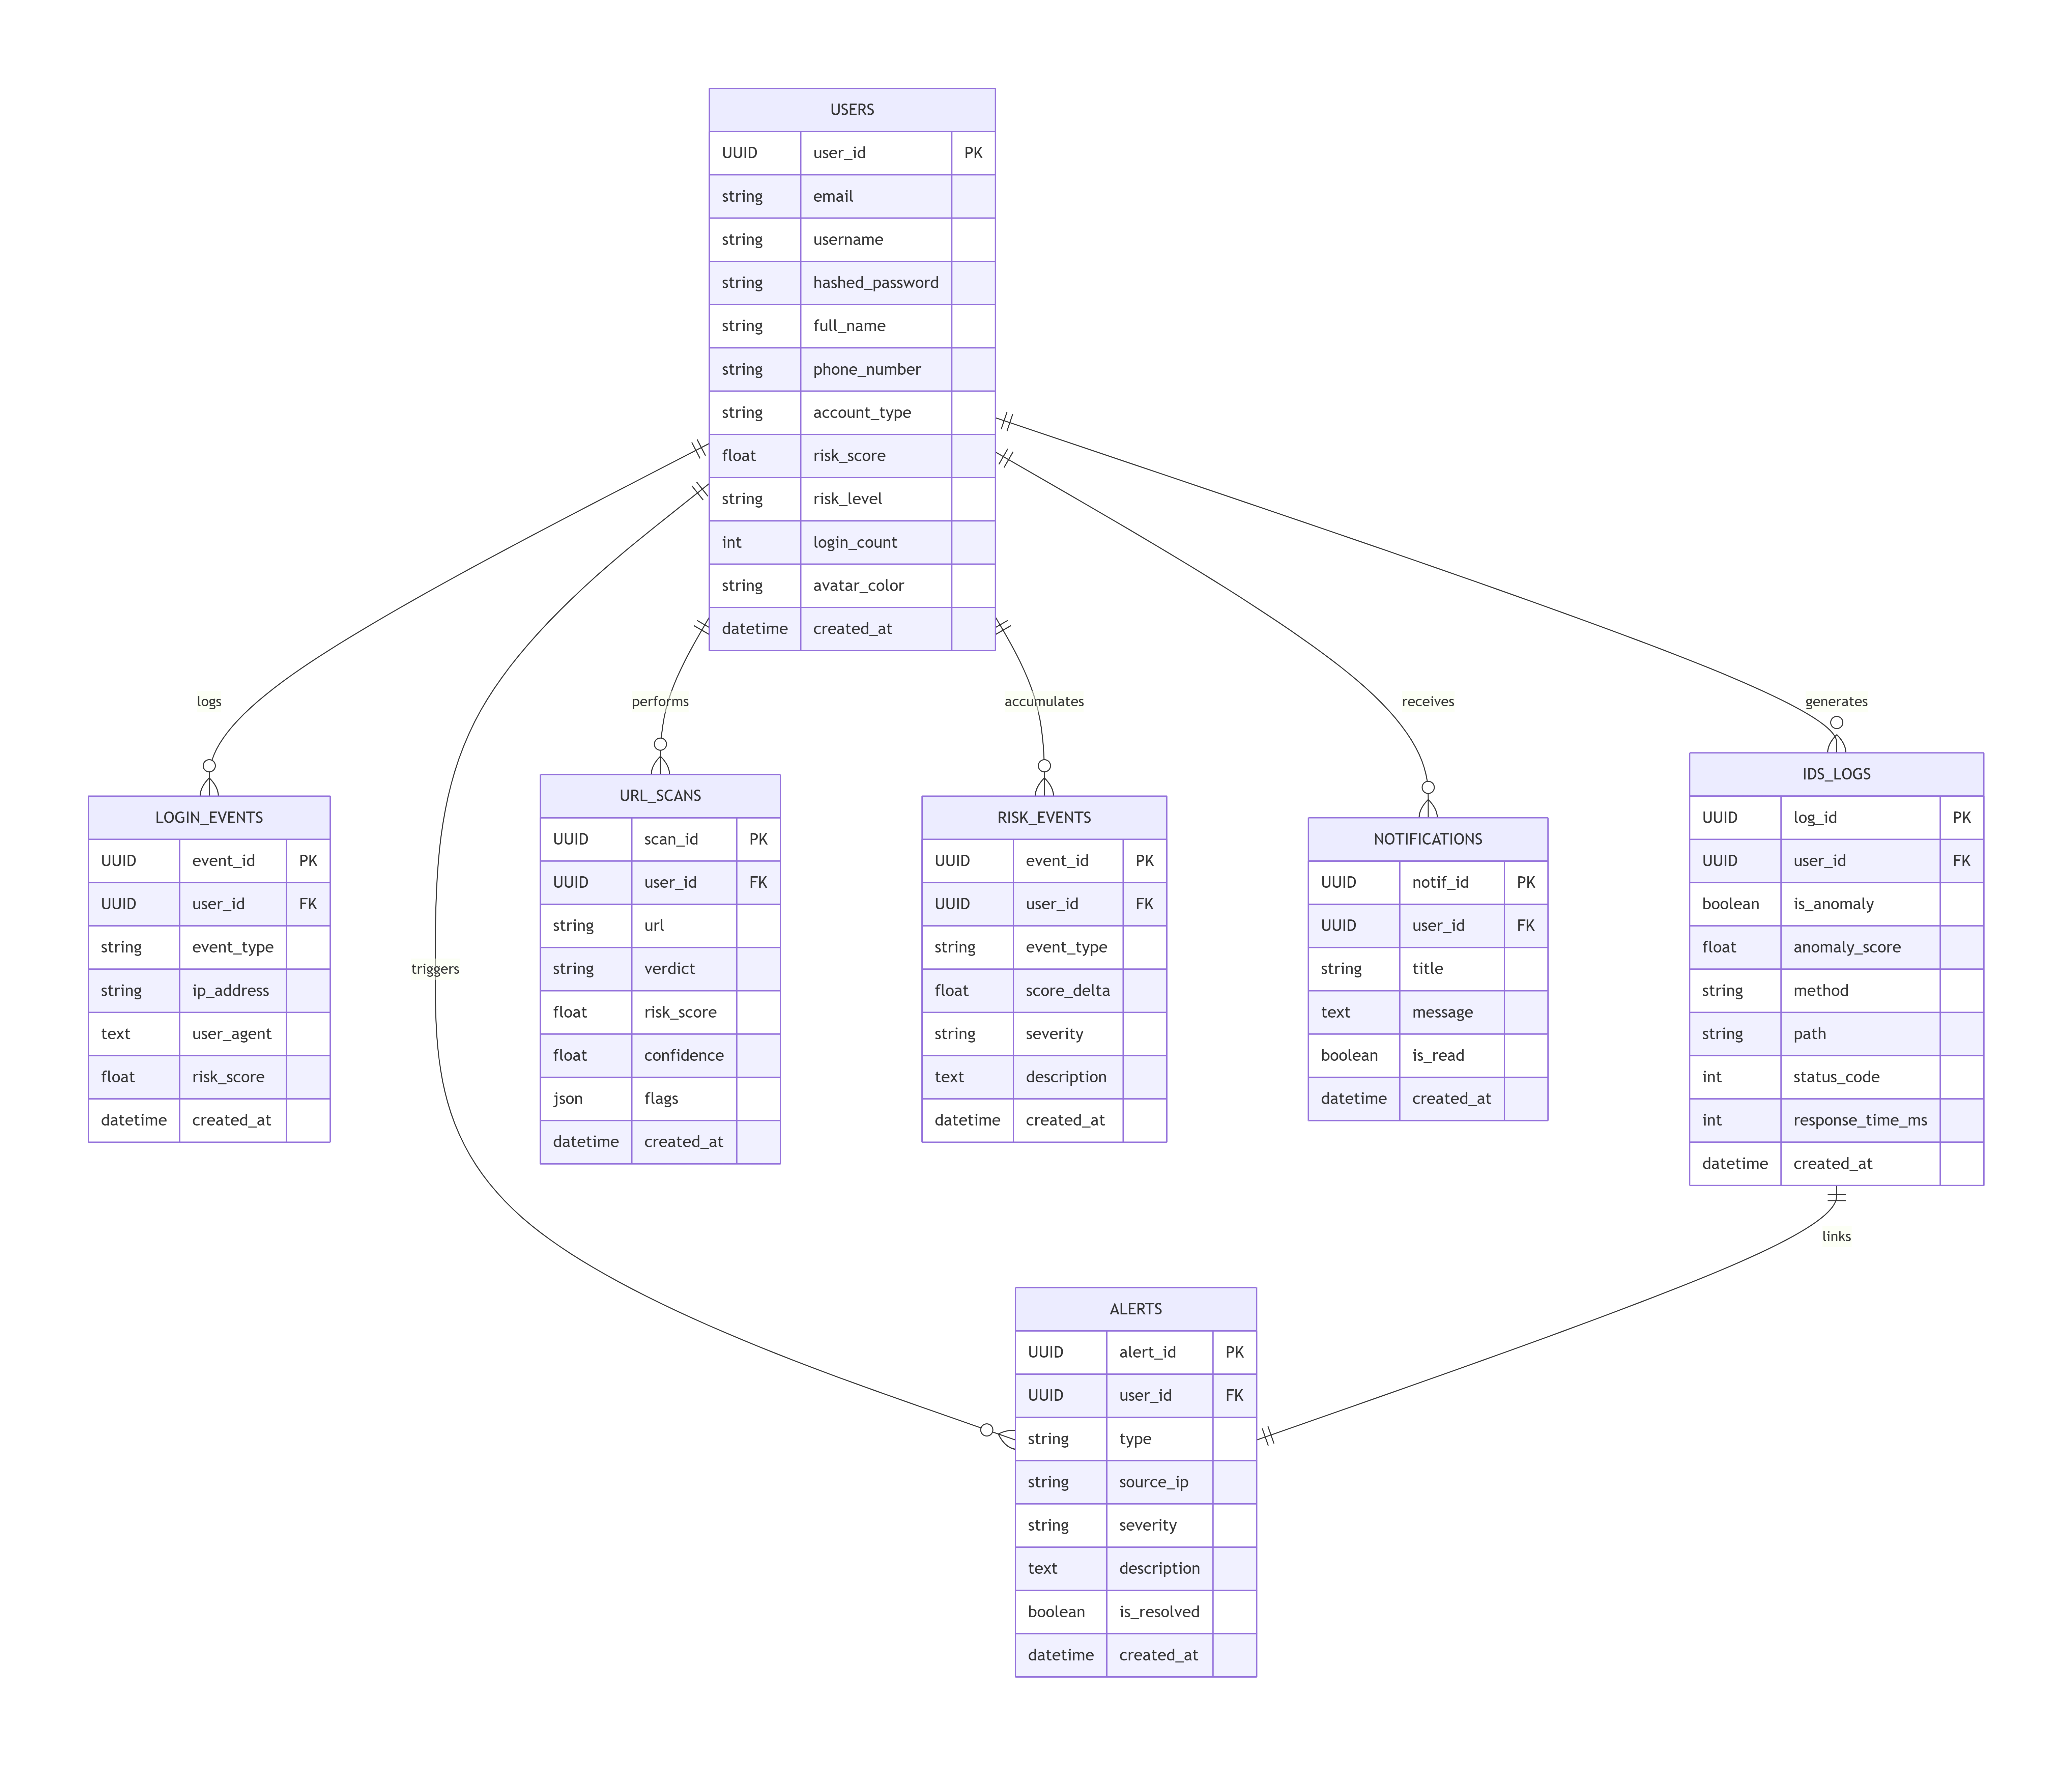
\includegraphics[width=\linewidth,height=0.75\textheight,keepaspectratio]{er_new}
    \caption{SmartSec --- Entity Relationship (ER) Diagram}
    \label{fig:er}
\end{figure}
\FloatBarrier

\noindent The \textbf{users} table is the central entity. It stores account credentials, profile information, current risk score, risk level, login statistics, and a JSONB field for user-configurable security settings. A single user has one-to-many relationships with all six other tables via the \texttt{user\_id} foreign key. The \textbf{login\_events} table records every authentication attempt with IP address, event type, risk score, and risk flags. The \textbf{ids\_logs} table stores ML model inference results. The \textbf{url\_scans} table stores phishing analysis verdicts with full feature breakdowns in JSONB. The \textbf{risk\_events} table maintains the risk scoring audit trail. The \textbf{notifications} and \textbf{alerts} tables handle in-app and email alert records respectively.

\section{Class Diagram (UML)}
The UML Class Diagram represents the object-oriented structure of the SmartSec backend service layer.

\begin{figure}[H]
    \centering
    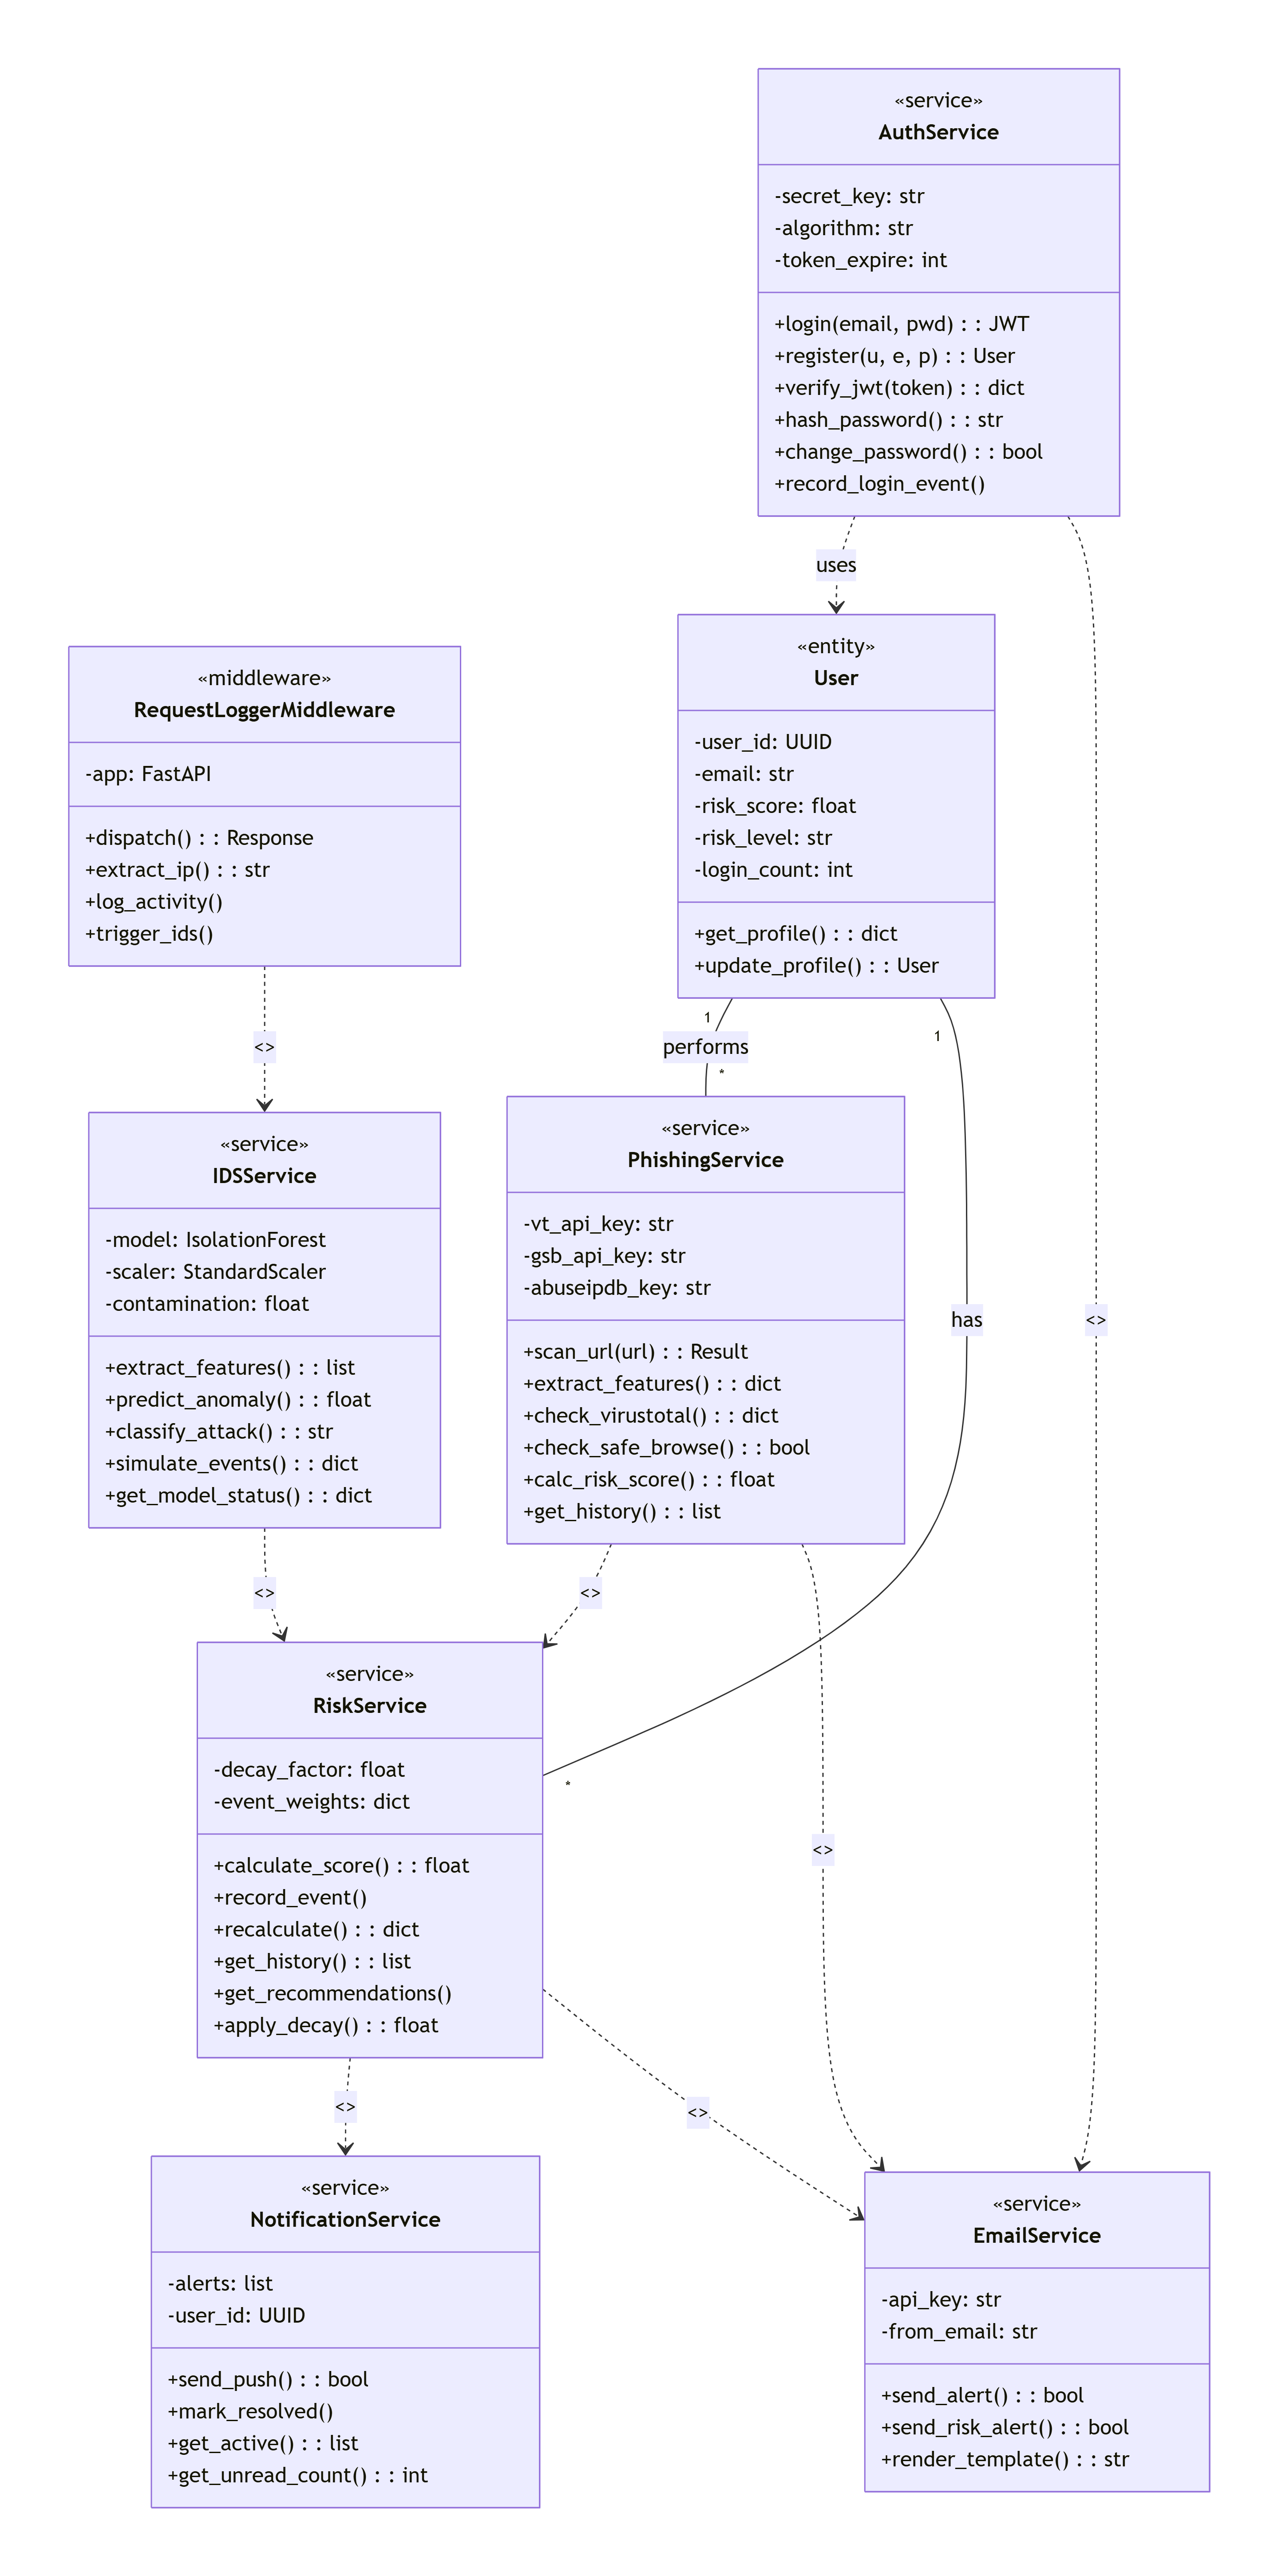
\includegraphics[width=\linewidth,height=0.75\textheight,keepaspectratio]{uml_new}
    \caption{SmartSec --- UML Class Diagram}
    \label{fig:class}
\end{figure}
\FloatBarrier

\noindent The seven core service classes are: \textbf{AuthService} (password hashing, JWT management, login risk assessment), \textbf{IDSService} (IsolationForest model lifecycle and inference), \textbf{PhishingService} (19-signal heuristics and three threat API clients), \textbf{RiskService} (weighted event scoring with 8\% daily exponential decay), \textbf{EmailService} (Resend API HTML alert delivery), \textbf{NotificationService} (in-app notification CRUD), and \textbf{DashboardService} (cross-module data aggregation).

\section{Activity Diagram}
The Activity Diagram illustrates the complete user workflow through the SmartSec platform from login to security action and notification delivery.

\begin{figure}[H]
    \centering
    \includegraphics[width=0.72\linewidth,height=0.82\textheight,keepaspectratio]{activity_new}
    \caption{SmartSec --- Activity Diagram}
    \label{fig:activity}
\end{figure}
\FloatBarrier

\noindent The flow begins with authentication (login or register). After a valid JWT is issued, the user lands on the Security Dashboard. From there, three parallel paths are available: IDS Analysis (run simulation, detect anomaly), Phishing Detection (submit URL, get multi-API verdict), or Risk/Profile Management (view risk breakdown, update settings). Each security action with a High or Critical outcome triggers the Risk Engine as a side-effect, updating the user's score, creating an in-app notification, and dispatching an automated email alert via the Resend API. The user is then returned to the dashboard, completing the activity cycle.

\section{Database Design}

The database uses PostgreSQL 15+ hosted on Supabase. All primary keys are UUID type generated by \texttt{gen\_random\_uuid()}. All timestamps use \texttt{timestamptz} with \texttt{DEFAULT now()} for timezone-aware audit records.

\begin{table}[H]
\centering
\caption{Core Database Tables --- SmartSec Platform}
\begin{tabular}{|p{3.5cm}|p{8cm}|p{2.5cm}|}
\hline
\textbf{Table} & \textbf{Key Columns} & \textbf{Linked To} \\
\hline
users & id, username, email, hashed\_password, risk\_score, risk\_level, user\_settings (JSONB) & --- (central) \\
\hline
login\_events & user\_id, event\_type, ip\_address, risk\_flags, created\_at & users \\
\hline
ids\_logs & user\_id, is\_anomaly, anomaly\_score, features (JSONB) & users \\
\hline
url\_scans & user\_id, url, verdict, risk\_score, confidence, features (JSONB) & users \\
\hline
risk\_events & user\_id, event\_type, severity, score\_delta, description & users \\
\hline
notifications & user\_id, title, message, type, is\_read & users \\
\hline
alerts & user\_id, type, is\_resolved, created\_at & users \\
\hline
\end{tabular}
\end{table}

\section{Input / Output Design}

\begin{table}[H]
\centering
\caption{Input Design for SmartSec System}
\begin{tabular}{|p{3.5cm}|p{4cm}|p{4cm}|}
\hline
\textbf{Input} & \textbf{Fields} & \textbf{Validation} \\
\hline
User Registration & Username, Email, Password & Unique email, min 8-char password \\
User Login & Email, Password & Valid credentials, bcrypt verify \\
OAuth Login & Google/GitHub token & Valid Supabase OAuth callback \\
URL Scan & URL string & Non-empty, max 2048 chars \\
IDS Simulation & Traffic count (int) & Min 1, max 1000 samples \\
Profile Update & Name, bio, location & Optional, max lengths enforced \\
\hline
\end{tabular}
\end{table}

\begin{table}[H]
\centering
\caption{Output Design for SmartSec System}
\begin{tabular}{|p{3.5cm}|p{5cm}|p{3cm}|}
\hline
\textbf{Output} & \textbf{Description} & \textbf{Visualisation} \\
\hline
Security Dashboard & Live stats: scans, anomalies, risk level, 7-day chart & Cards + AreaChart \\
IDS Report & Classification, confidence, recent anomaly table & Table + PieChart \\
Phishing Verdict & Safe/Suspicious/Phishing, risk score, 19 signal flags & Verdict card \\
Risk Score View & Gauge, 30-day timeline, category breakdown & RadarChart + Gauge \\
Notification Bell & Live unread count, dropdown alert list & Badge + dropdown \\
Login Audit & Full history: timestamp, IP, risk flags & Paginated table \\
\hline
\end{tabular}
\end{table}
